\chapter{A Dynamic Model for Co-located Collaboration}
\label{chapter:dynamic_model}
\minitoc

\section{Introduction}
The Altered Human Joystick metaphor is based on a 
we designed a dynamic model which integrates real world information into the virtual navigation control in the aim of providing a general framework for co-located collaboration by supporting both consistent and individual modes and also fluent transition between them.

DYNAMIC model: DYnamic NAvigation Model for Immersive Collaboration.  which is a more advanced version of the Altered Human Joystick metaphor.


% -------------------------------------------------------------------------------------------------

\section{Motivation and Objective}

Natural and intuitive hand-free navigation. Infinite navigation within limited physical workspace.

Aware of physical environment, guidance to avoid fixed and mobile obstacles (wall screen, other user, haptic arm, etc.). A generic model: not dependent on system configuration
 
extensible in terms of user number and control method

More flexible bi-directional control of navigation, friction, pseudo-haptic feedback

One user should not be disturbed by other users when in a stable state

Integrating constrains from virtual world into the navigation control.

% -------------------------------------------------------------------------------------------------


\section{Concepts}

\subsection{Virtual Vehicle}
This dynamic model is based on a \textit{virtual vehicle} as described in Section~\ref{sec:navigation}. The idea is that each user is on board a personal vehicle that allows virtual navigation in 3D space under user's control. From a mathematical point of view, this vehicle is just a mobile spatial reference frame (as explained in Section~\ref{sec:srframe}) which helps to map user's physical workspace to its counterpart in the virtual world. Here we borrow some definitions from the Immersive Interactive Virtual Cabin (IIVC) model (Figure~\ref{fig:5_iivc}) that can help to describe the virtual vehicle for navigation:

\begin{itemize}
\item The \textit{stage} is a virtual representation of the physical workspace;
\item The \textit{conveyor} is the integration frame of the stage into the virtual world. This conveyor has its own position, orientation and scale in the virtual world coordinate system, and the stage is linked to the conveyor with position, orientation, and scale offsets.
\end{itemize}

\begin{figure}[htb]
  \centering
  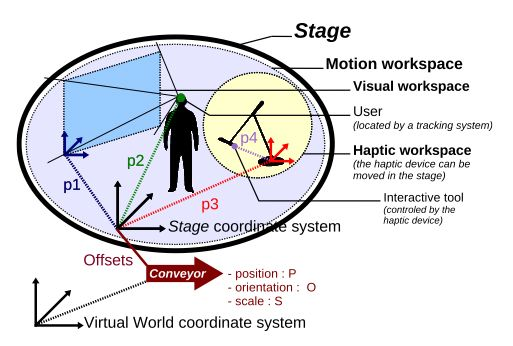
\includegraphics[width=.7\textwidth]{figures/ch5/IIVC}
  \caption{\label{fig:5_iivc}The IIVC model: the conveyor carries the stage with its workspaces in the virtual world \citep{Fleury2010Generic}.}
\end{figure}

The virtual vehicle is just a special type of conveyor that is superimposed with user's avatar in the virtual world, so from user's first person viewpoint, the vehicle is always situated underneath user's current location, or we can say that the user is on board his/her personal vehicle in the virtual world in order to navigate. As illustrated in Figure~\ref{fig:5_vehicle}, the user navigates as the vehicle moves forward in the virtual world (the stage is also ``carried" by the vehicle). The vehicle has a constant orientation offset with the stage, but the position offset changes as the user moves in the real environment. In this way the rotation is always centered around user's avatar position no matter his/her location with respect to the physical workspace.

\begin{figure}[htb]
  \centering
  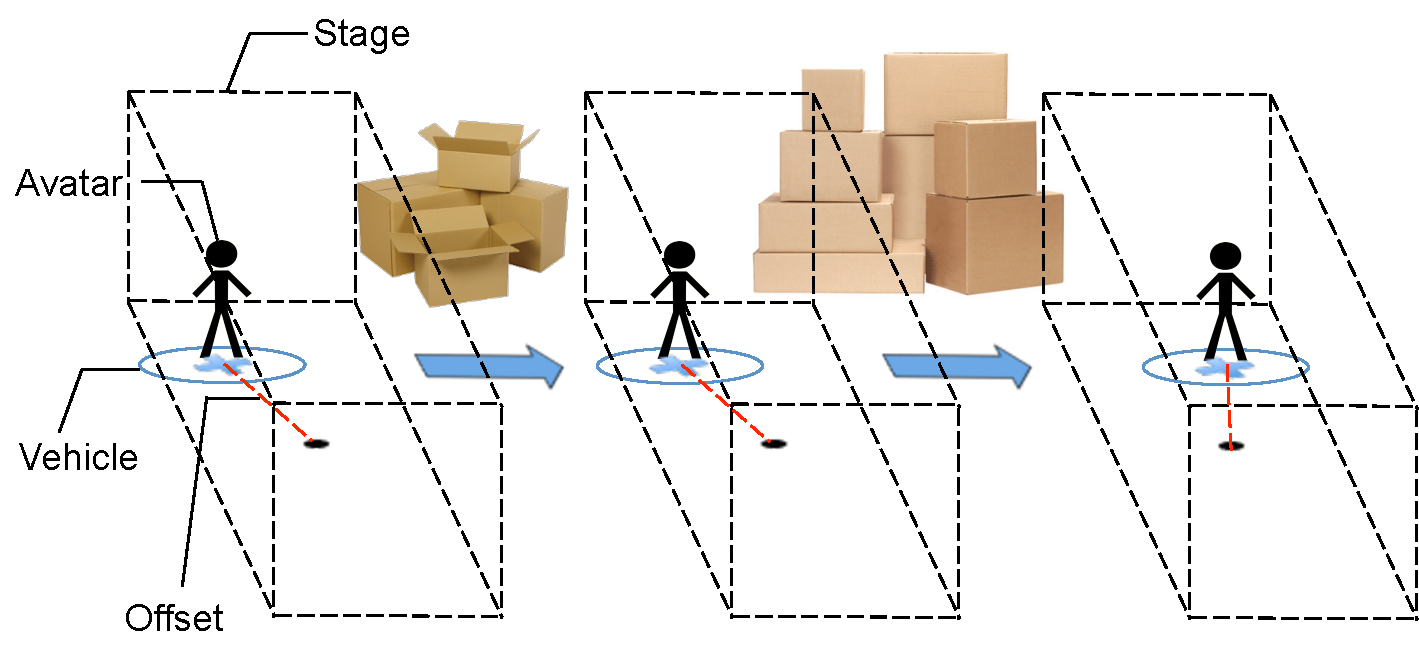
\includegraphics[width=.9\textwidth]{figures/ch5/vehicle}
  \caption{\label{fig:5_vehicle}Illustration of virtual vehicle based navigation.}
\end{figure}

We name this reference frame as a vehicle instead of conveyor mainly for two reasons: first, rate control navigation techniques provide similar navigation experience as we drive or pilot vehicles in the real world; second, we can reproduce some ``realistic" vehicle-based navigation behaviors (e.g. collisions, frictions) by adding constrains to the virtual vehicle without physicalize the whole virtual scene.

As a summary, the virtual vehicle provides a standard abstraction which facilitates the design of rate control navigation techniques, we just need to concentrate on how to control the vehicle. This conceptual model also makes it easier to understand user's velocity perception within immersive displays. When the user can move in the physical workspace, the navigation velocity perceived by the user is the sum of the virtual vehicle's velocity and user's velocity in the real workspace: 

\begin{equation}
\overrightarrow{v_{perceived}} = \overrightarrow{v_{vehicle}} + \overrightarrow{v_{user}}
\end{equation}

The virtual vehicle along with the IIVC model can be easily adapted to manage multiple co-located users in immersive virtual environments. Each user has his/her own copy of stage and virtual vehicle (Figure~\ref{fig:5_multi_vehicle}) which allows individual navigation. Group navigation can also be achieved by merging all the stages and giving the control of all vehicles to a leader. 

\begin{figure}[htb]
  \centering
  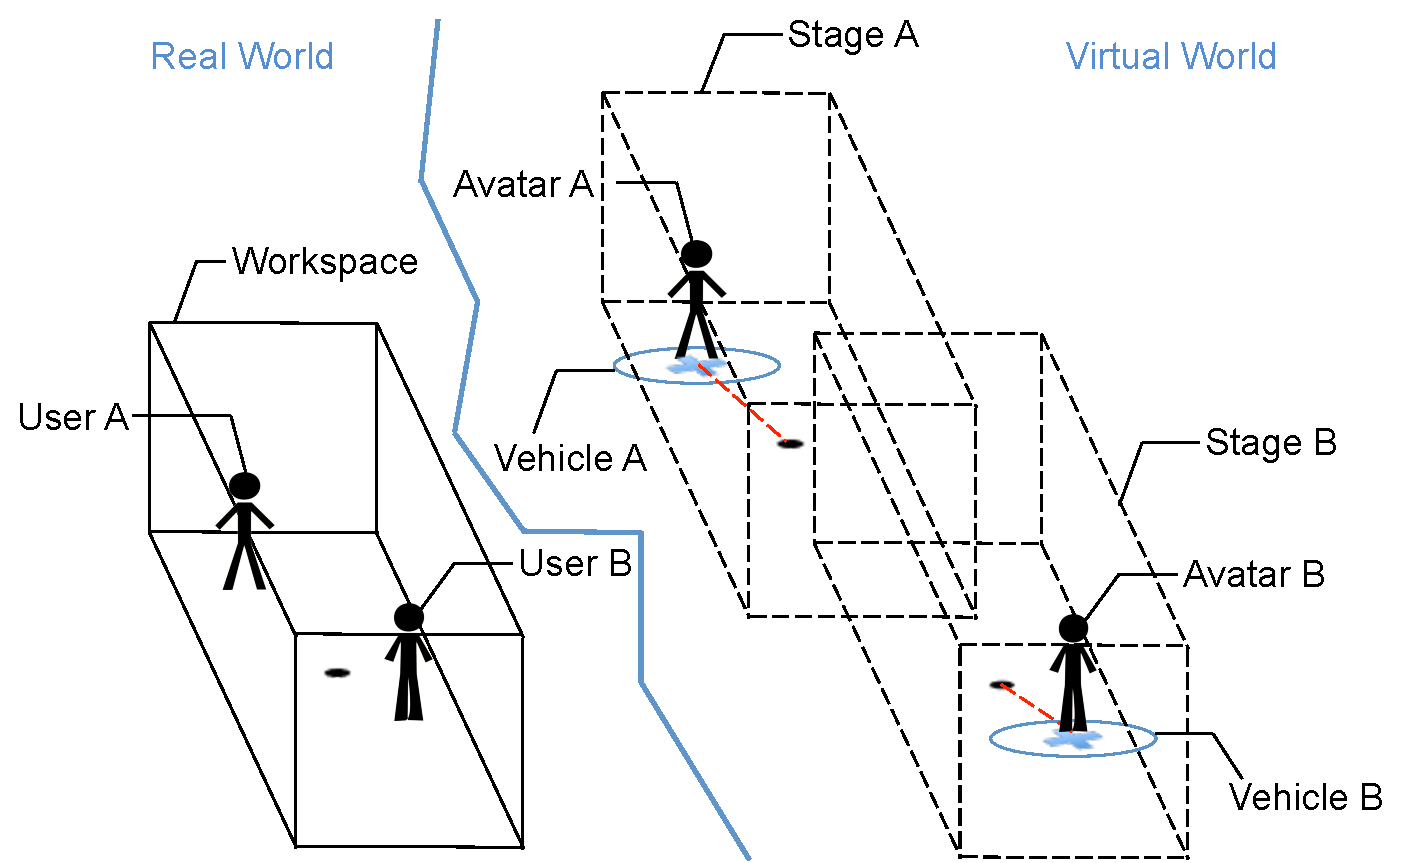
\includegraphics[width=.9\textwidth]{figures/ch5/multi_vehicle}
  \caption{\label{fig:5_multi_vehicle}Illustration of virtual vehicle based navigation.}
\end{figure}


\subsection{Transfer Function}
Rate control navigation metaphors are mainly characterized by their transfer functions. A transfer function (TF) transforms user's input into a change of the virtual vehicle's kinematic state. User inputs can be in form of device events (e.g. joystick buttons), gestures and postures controllers map button events  

- definition
- classic examples
- the one for dynamic model


\subsection{Potential Field}
In the domain of robotics, potential force field is one of the algorithms that can be used to guide a robot to navigate over a field occupied by obstacles to get to a goal position. Generally, two kinds of potential fields lead to two different behaviors of the robot. An attractive field generates an action vector that points the robot toward the goal, while a repulsive field pushes the robot away from an obstacle.

Here, the goal is to keep the user away from all the obstacles when he/she moves around in the real workspace. So one way could be adding repulsive fields to each obstacle (screens and other users). Instead of directly pushing the user, we can apply an action vector to user's initial point. The final potential field will be the combination of the field of each obstacle. Since users can move around, so the final potential field will change accordingly. Take an example of user A (cf. Figure 1), the potential field will be the combination of repulsive field of each screen wall and of user B.

To take into consideration the physical surrounding of the navigating user, a \textbf{Solver} gathers information about physical obstacles and computes an optimal point based on a potential force field. Then we define a command point (where the user should be in the real world) which is linked with the optimal point, but they are not always superimposed. For example, the movements of one user change instantaneously the optimal point of another, to reduce this instability, we can restrict the velocity of control point so the influence is minimized. An \textbf{Inverse Model} computes an acceleration based on the difference between the command point and user's current configuration which helps to lead the user to that point.

\subsection{Virtual Constrains}
In addition to accelerations coming from real world, whether from user or the surrounding environment, another advantage of this navigation paradigm is that we can easily integrate constrains of the virtual world into the navigation model. For example, we can add artificial viscosity or friction to the vehicle so it will slow down with time goes by. Imagine two users moving together a virtual table to another place, in this case their vehicles are virtually connected by the table so they have mutual influences on each other's navigation control.

for example, we can apply an acceleration in the opposite direction of the vehicle's current velocity to simulate the viscosity of the virtual world. 


% -------------------------------------------------------------------------------------------------


\section{Implementation}
\subsection{Kinematic State}
Kinematics is a field of study which describes the motion of points and more complex objects without consideration of the causes of motion \citep{Beggs1983Kinematics}. It is the basic component of a physics engine for virtual simulation.

Instead of navigating by setting a user's position and orientation in the virtual world, we can also make use of other kinematic information such as velocity and acceleration to control user's virtual motion, especially in cases where we look for navigation sensations that are close to those we have in the physical world. 

\subsubsection{Representation}
We created a variable called \textit{kinematic state} (KS) to store all motion-related data of a given object. In 3D space, an object's KS usually contains two parts of information respectively for translation and rotation, except those of points (considered as particles) which have only positional information. Different components of an object's KS are listed in Table~\ref{tab:5_ks_components}.

\begin{table}[hbt]
\renewcommand{\arraystretch}{1.3}
\caption{Components of kinematic state}
\label{tab:5_ks_components}
\centering
\begin{tabular}{l l l}
  \hline
  Components & Translation Part & Rotation Part \\
  \hline
  Static configuration $c(p, q)$ & Position $p(x, y, z)$ & Orientation $q(w, x, y, z)$ \\
  Velocity $v(\overrightarrow{v}, q_{v})$ & Linear velocity $\overrightarrow{v}(v_{x}, v_{y}, v_{z})$ & Angular velocity $q_{v}$ \\
  Acceleration $a(\overrightarrow{a}, q_{a})$ & Linear acceleration $\overrightarrow{a}(a_{x}, a_{y}, a_{z})$ & Angular acceleration $q_{a}$ \\
  \hline
\end{tabular}
\end{table}


\subsubsection{State Update}
An object's KS changes constantly while moving in 3D space. The current KS can be updated by providing a new acceleration, or by directly designing a new static configuration. For example, we can accelerate a virtual object by injecting an acceleration on that object, this results in a corresponding velocity and configuration change. A real world entity such as a user's physical body also has a KS,

 The user also has a KS that is updated by tracking information in a different way than the vehicle.

\paragraph{Update by Acceleration}
The verlet integration is used to update the KS with a new acceleration.

For translation:

\[
\overrightarrow{p_{1}}=\overrightarrow{p_{0}}+\overrightarrow{v_{0}}\Delta t+\frac{1}{2}\overrightarrow{a_{0}}\Delta t^{2}
\]

\[
\overrightarrow{v_{1}}=\overrightarrow{v_{0}}+\frac{\overrightarrow{a_{0}}+\overrightarrow{a_{1}}}{2}\Delta t
\]

And for rotation, we choose to represent the orientation in quaternion for its convenience and simplicity, while angular velocity and acceleration are expressed separately according to euler angles:

\[
\omega_{1}=\omega_{0}+\frac{\dot{\omega_{0}}+\dot{\omega_{1}}}{2}\Delta t
\]

\[
q_{1}=q_{a}q_{v}q_{0}
\]

\[
q_{v}=\left(\cos(\frac{\Vert\omega_{0}\Vert\Delta t}{2}),\:\sin(\frac{\Vert\omega_{0}\Vert\Delta t}{2})\frac{\omega_{0}(x)}{\Vert\omega_{0}\Vert\Delta t},\:\sin(\frac{\Vert\omega_{0}\Vert\Delta t}{2})\frac{\omega_{0}(y)}{\Vert\omega_{0}\Vert\Delta t},\:\sin(\frac{\Vert\omega_{0}\Vert\Delta t}{2})\frac{\omega_{0}(z)}{\Vert\omega_{0}\Vert\Delta t}\right)
\]

\[
q_{a}=\left(\cos(\frac{\Vert\dot{\omega_{0}}\Vert\Delta t}{2}),\:\sin(\frac{\Vert\dot{\omega_{0}}\Vert\Delta t}{2})\frac{\dot{\omega_{0}}(x)}{\Vert\dot{\omega_{0}}\Vert\Delta t},\:\sin(\frac{\Vert\dot{\omega_{0}}\Vert\Delta t}{2})\frac{\dot{\omega_{0}}(y)}{\Vert\dot{\omega_{0}}\Vert\Delta t},\:\sin(\frac{\Vert\dot{\omega_{0}}\Vert\Delta t}{2})\frac{\dot{\omega_{0}}(z)}{\Vert\dot{\omega_{0}}\Vert\Delta t}\right)
\]


\paragraph{Update by Configuration}
(in form of a 4x4 matrix)



\subsection{Structure}

python

class schema

sequential graph

% -------------------------------------------------------------------------------------------------

\section{Mode Switching}
state machine


% -------------------------------------------------------------------------------------------------

\section{Parameter Setting}


% -------------------------------------------------------------------------------------------------

\section{Conclusion}
We need a model of human for reaction of acceleration.